\subsection{Schnyder-Wood-Fluss}

Um einen Schnyder Wood zu erhalten folgen wir \cite{felsner04}.\
Wir betrachten den Primal-Dual Graphen $G+G^*$ eines planen Graphen $G$. Hier ist $G^*$ der schwache duale Graph zusammen mit einer Halbkante ins äussere Gebiet von jeder inzidenten Kante aus. Die Menge der Knoten von $G+G^*$ besteht aus Knoten-Knoten, Kanten-Knoten und Gebiets-Knoten, mit Kanten in $G+G^*$, sowohl zwischen inzidenten Kanten und Knoten, als auch Kanten und Gebieten in $G$. Somit ist $G+G^*$ bipartit. Falls wir einen Knoten $f_\infty$ für das äussere Gebiet einsetzten und die Halbkanten verlängern sprechen wir vom Abschluss von $G+G^*$. Wir bezeichnen diesen mit $\tilde{G}$.\\
Sei $G=(V,E)$ ein Graph und $\alpha:V\mapsto\mathbb{N}$ eine Funktion auf $G$. Eine $\alpha-Orientierung$ ist eine Orientierung auf $G$, sodass der Ausgrad eines jeden Knoten $\alpha(v)$ entspricht. Das folgende Theorem stammt ebenfalls aus \cite{felsner04lattice}.

\begin{theorem}\label{alpha_bij}
Sei $G$ ein planer Graph mit Aufhängungen $\{a_1,a_2,a_3\}$, dann sind die folgenden Strukturen in Bijektion:
\begin{itemize}
\item Die Schnyder Wälder auf $G$.
\item Die Schnyder Wälder auf dem (schwachen) dualen Graph $G^*$.
\item Die $\alpha_{s}-Orientierungen$ des Abschlusses von $G+G^+$ mit $\alpha_s(v) = 3$ für jeden Knoten- und Gebiets-Knoten,  $\alpha_s(e) = 1$ für jeden Kanten-Knoten und  $\alpha_s(f_\infty) = 0$.
\end{itemize}
\end{theorem}

Fusy zeigt in \cite{fusy07} im Zuge der Untersuchung spezifischer $\alpha$-Funktionen, dass sich $\alpha_s$-Orientierungen von $G+G^*$ in linearer Zeit berechnen lassen.\\

Machen wir uns also an die Konstruktion eines Netzwerks $\mathcal{N}_S$ mit einer Quelle und Senke, sodass eine zulässige Lösung $\varphi$ einer $\alpha_s-Orientierung$ von $\tilde{G}$ entspricht, und somit auch einen Schnyder Wald auf $G$ liefert. Besonderes Augenmerk ist hier auf die Möglichkeit einer späteren Kombination mit einem FAA Fluss gelegt, um ein Zwei-Fluss-Problem zu erstellen, und nicht unbedingt auf Effizienz.\

Wie oben schon erwähnt ist $\tilde{G}$ bipartit, Kanten-Knoten haben Grad 4, Knoten-Knoten Grad $deg(v)$ und Gebiets-Knoten Grad $|f|$. Für eine $\alpha_s$-Orientierung muss jeder Kanten-Knoten Ausgrad 1, jeder Knoten-Knoten Eingrad $deg(v)-3$ und jeder Gebiets-Knoten Eingrad $|f|-3$ haben. Die Kanten-Knoten am äusseren Gebiet sind in $\tilde{G}$ immer nach aussen orientiert. Somit müssen wir nur die inneren Kanten-Kanten $E_{in}$ betrachten. \

\begin{figure}[h]
	\centering
  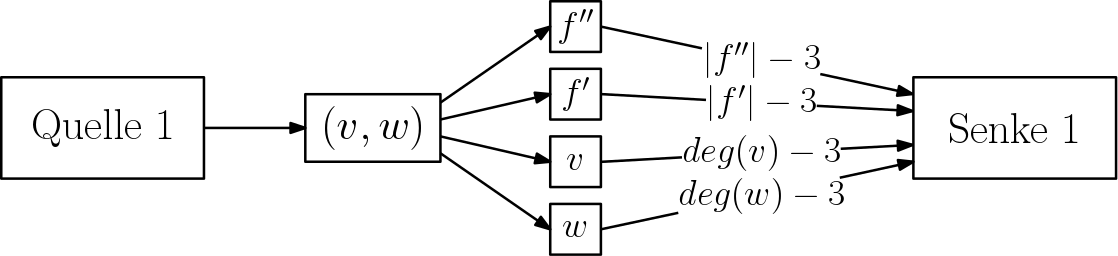
\includegraphics[width=0.9\textwidth]{schnyder_flow.png}
\end{figure}

Sei $\mathcal{N}_S$ ein Netzwerk mit jeweils einer Quelle $s$ und Senke $t$, Kanten von der Quelle zu jedem $e \in E_{in}$ mit Kapazität 1, Kanten von den Kanten-Knoten $e$ zu inzidenten Knoten-Knoten $v$ und (inneren) Gebiets-Knoten $f \in F_{in}$ in $G$ ebenfalls mit Kapazität 1, Kanten von $f \in F_{in}$ zur Senke mit Kapazitäten $|f|-3$, Kanten von den (inneren) Knoten-Knoten $v \in V_{in} = V \setminus \{a_1,a_2,a_3\}$ zur Senke mit Kapazitäten $deg(v)-3$ und Kanten von den Aufhängungen $a_i$ zur Senke mit Kapazitäten $deg(v)-2$. Die letzte Kapazität resultiert aus dem Fakt, dass die Halbkante in $G+G^*$ immer nach aussen orientiert ist und wir somit nur noch zwei andere Kanten nach aussen orientieren müssen.

Der Bedarf des Netzwerkes entspricht der Anzahl der inneren Kanten von $G$. Sei nun $\varphi$ eine zulässige ganzzahlige Lösung, dann hat jeder Kanten-Knoten $e$ Ausgrad 1. Der Fluss entlang einer Auskante von $e \in E_{in}$ in $\mathcal{N}_S$ entspricht dann genau der hin zu $e$ orientierten Kante in $G+G^*$ und die Knoten-Knoten und Gebiets-Knoten haben genau $deg(v)-3$ bzw. $|f|-3$ zu ihnen hin orientierte Kanten. Eine zulässiger ganzzahliger Fluss kodiert also eine $\alpha_s$-Orientierung auf $G+G^*$. Somit liefert uns $\varphi$ nach Theorem \ref{alpha_bij} auch einen Schnyder Wald auf $G$.

\subsection{FAA-Fluss}\label{fas-flow}

Um ein FAA für einen planaren Graphen $G$ zu erhalten müssen wir jedem Gebiet $f \in F$ genau drei Ecken und $|f|-3$ flache Winkel zuordnen und jeder Knoten darf maximal einem Gebiet zugeordnet werden, also in diesem flach sein. Falls eine Einbettung und die Aufhängungen $\{a_1,a_2,a_3\}$ gegeben sind, müssen wir jedem inneren Gebiet $f \in F_{in}$ drei Ecken und $|f|-3$ flache Winkel zuweisen und jeder innere Knoten $v \in V_{in}$ darf maximal einem Gebiet zugeordnet werden. Wir konstruieren ein Netzwerk für den zweiten Fall, dass sich leicht verallgemeinern lässt.\

Sei also wieder $\mathcal{N}_F$ ein Netzwerk mit einer Quelle und Senke, einem Knoten für jeden inneren Winkel $(f,v)$ für $v\in V, f \in F_{in}$, Knoten für alle inneren Gebiete $f$ und alle inneren Knoten $v$. Von der Quelle existiert eine Kante mit Kapazität 1 zu jedem inneren Winkel $(f,v)$, von jedem inneren Winkel $(f,v)$ jeweils eine Kante zu $f$ und zu $v$ mit Kapazität 1, von jedem inneren Gebiet $f$ eine Kante mit Kapazität 3 zur Senke und zuletzt noch eine Kante von jedem inneren Knoten $v$ zur Senke mit Kapazität 1.

\begin{figure}[h]
	\centering
  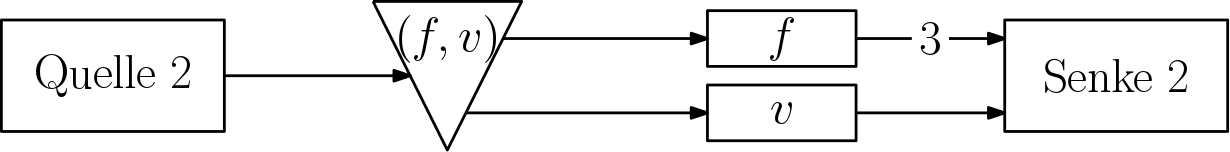
\includegraphics[width=0.8\textwidth]{faa_flow.png}
\end{figure}


Der Bedarf des Netzwerks ist $\sum_{f \in F_{in}}{|f|}$, die Anzahl der inneren Winkel von $G$. Sei $\varphi$ ein zulässiger ganzzahlige Fluss, dann entspricht Fluss auf einer Kante $((f,v),f)$ einer Ecke, von $f$ und Fluss auf $((f,v),u)$ einem flachen Winkel, zur Vereinfachung sprechen wir im Weitern auch von Ecken- respektive Zuweisungs-Fluss. Somit wird jeder innere Winkel entweder dem Gebiet zugewiesen oder als Ecke ausgezeichnet und es kann nur jeweils ein Winkel an jedem inneren Knoten zugewiesen werden. Somit respektiert $\varphi$ die Bedingungen aus Definition \ref{faa} und es existieren nur dann FAAs auf $G$, falls mindestens eine ganzzahlige Lösung auf $\mathcal{N}_F$ existiert.

\begin{remark}

Das oben konstruierte Netzwerk zur Bestimmung von FAAs lässt sich auch als Zwei-Fluss Problem konstruieren, wenn wir für Ecken- und Zuweisungs-Fluss getrennte Quellen und Senken einführen. Der Bedarf des Ecken-Flusses ist dann $3|F_{in}|$ und der Bedarf des Zuweisung-Flusses $\sum_{f \in F_{in}}{|f|-3}$.

\begin{figure}[h]
	\centering
  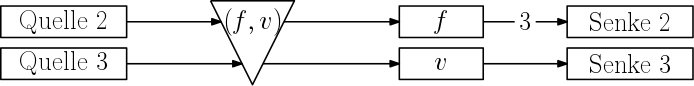
\includegraphics[width=0.8\textwidth]{faa_2_flow.png}
\end{figure}

Eine zulässige ganzzahlige Lösung $\varphi = (\varphi_2,\varphi_3)$ entspricht dann wieder einem FAA auf $G$, da aus der Ganzzahligkeit folgt, dass ein Winkel entweder von $\varphi_2$ oder $\varphi_3$ genutzt wird und somit eine Definition \ref{fad} respektierende Beschriftung der Winkel vorliegt.

\end{remark}

\subsection{Graphen mit wenigen FAAs oder Schnyder Woods}

Sei $G$ ein planer Graph mit nur polynominell vielen Schnyder Woods bzw. FAAs, dann liefern die oben angegebenen Algorithmen auch einen polynominellen Ansatz zur Bestimmung einer SLTR. Wir \\
TODO

